\documentclass[conference]{IEEEtran}
\usepackage[utf8]{inputenc}
\usepackage{url}
\usepackage{amsmath}
\usepackage{amssymb}
\usepackage{graphicx}
\usepackage[colorlinks=true, linkcolor=blue, citecolor=blue, urlcolor=blue]{hyperref}


\begin{document}

\title{Seminar - Collective navigation of a multi-robot system in an unknown environment}
\author{\IEEEauthorblockN{Gregor Germerodt}
\IEEEauthorblockA{Hochschule Trier - Trier University of Applied Sciences\\
E-Mail: grgr3403@hochschule-trier.de\\
Themensteller und Betreuer: Prof. Dr. Jürgen Graf\\
Cognitive Systems and Robotics}}

\maketitle


\begin{abstract}
Diese Arbeit stellt eine Zusammenfassung der Arbeit von Olcay (2020) dar. Alle Inhalte basieren
auf diese Arbeit \cite{Olcay.2020} und dessen referenzierten Quellen wurden 
an benötigten Stellen übernommen.

Vorgestellt werden verschiedene Verfahren für die Bewegung von Robotern in unbekannten Umgebungen,
zur Kollisionsvermeidung und Zielerreichung anhand virtueller Kräfte. Zuerst werden die Verfahren
für einen einzelnen Roboter erklärt und diese dann mit Hilfe eines Kommunikationsnetzwerk auf 
ein Multi-Roboter-System erweitert.
\end{abstract}

\section{Introduction}
Multi-robot systems, such as autonomous robots collaborating in a swarm, 
offer applications in unknown environments like mapping, exploration, or 
rescue missions \cite{Stormont.null}. 
To ensure collision-free paths, this work addresses 
collective navigation under limited sensor and communication ranges. To 
enhance system robustness, a nature-inspired swarm behavior is applied, 
based on three simple rules: cohesion, separation, and alignment 
\cite{Reynolds.1987}. 
While global motion planning assumes an initial map with static obstacles, 
this work focuses on local motion planning that can dynamically respond 
to environmental changes. Instead of using Simultaneous Localization and 
Mapping (SLAM), where robots build a map while estimating their own 
position, this approach relies on a decentralized, potential field-based 
navigation method using only local sensor data and neighbor-to-neighbor 
communication. This enables the robots to make early, collective decisions 
for collision avoidance while ensuring scalability and flexibility of 
the system.

\section{Theoretical background}
Im betrachteten Multi-Roboter-System werden die Roboter als Punktmassen 
(d.h. ohne räumliche Ausdehnung, nur durch Position und Massepunkt) in einer 
zweidimensionalen Umgebung modelliert. Die Systemdynamik basiert auf potenzialfeldbasierten 
Kräften, wobei nur die Position und Geschwindigkeit jedes Roboters $i$ betrachtet werden,
$(p_i, v_i) \in \mathbb{R}^2 \times \mathbb{R}^2$.
Die Bewegungsdynamik jedes Roboters $i$ wird durch folgende Differentialgleichungen beschrieben:
\begin{equation}
    \dot{p}_i = v_i
    \label{eq:1}
\end{equation}
\begin{equation}
    \dot{v}_i = u_i
    \label{eq:2}
\end{equation}
Die Position des Roboters ändert sich also mit seiner Geschwindigkeit (1) und diese wiederum 
durch eine Steuerkraft (2).
Jeder Roboter kann nur mit benachbarten Robotern innerhalb eines festen 
Kommunikationsradius $r_c$ bidirektional interagieren. Die zeitabhängige und ungerichtete 
Nachbarschaft ist definiert durch
\begin{equation}
    \mathcal{N}_i^\alpha = \{ j \in \mathcal{V} \; | \; \| p_j - p_i \| < r_c \}
    \label{eq:3}
\end{equation}
mit $\mathcal{V} = \{1, \ldots, N\},\ N \in \mathbb{N}$, die Menge aller Roboter.
Um Schwarmverhalten zu erzeugen, werden zwischen zwei Robotern Distanzwerte berechnet, 
welche Abweichungsenergie, den Grad der Interaktion und Verbundenheit bestimmen ((4) bis (6)).

Die Steuerkraft $u_i$ eines Roboters $i$ wird über die Gleichung
\begin{equation}
    u_i = u_i^\alpha + u_i^\beta + u_i^\gamma
    \label{eq:4}
\end{equation}
berechnet, wobei $u_i^\alpha$ für Schwarmverhalten, $u_i^\beta$ für 
Hindernisvermeidung und $u_i^\gamma$ für Navigation sorgt. Das Schwarmverhalten 
$u_i^\alpha$ setzt sich aus Abstands- und Geschwindigkeitsanpassungen zu Nachbarn (8) 
sowie deren Wirkstärke in Abhängigkeit vom Abstand ((9) bis (10)) zusammen.

Die Hindernisvermeidung $u_i^\beta$ wird definiert durch die Hindernispunkte 
die ein Roboter erkennt (11), wie stark er von ihnen 
abgestoßen wird (12) und wie diese Abstoßungskraft in Abhängigkeit vom Abstand 
berechnet wird (13). Die Steuerkraft für die Navigation $u_i^\gamma$ sorgt für eine Anziehung
des Roboters zum Ziel.


\subsection*{The problem statement}
Viele bestehende Navigationsansätze für Multi-Roboter-Systeme basieren auf künstlichen 
Potenzialfeldern, bei denen Roboter von Zielpunkten angezogen und von Hindernissen 
abgestoßen werden. Ein zentrales Problem dieser Methoden sind jedoch lokale Minima, in 
denen sich Anziehungs- und Abstoßungskräfte ausgleichen und Roboter feststecken. 
Verfahren für einzelne Roboter, wie kamera- oder eliminationsbasierte Ansätze stoßen bei 
schwierigen Umweltbedingungen oder bei Hinderniskonfiguationen an ihre Grenzen.
Weiterhin ist die Herausforderung für Multi-Roboter-Systeme, kollisionsfrei und 
effizient in unbekannten und komplexen Umgebungen zu navigieren, trotz begrenzter 
Sensor- und Kommunikationsreichweiten. 
Aus diesem Grund, befasst sich diese Studie mit Kommunikation und Bewegungsplanung mehrerer Roboter,
wobei Rausch-Effekte, Zeitverzögerung oder Paketverlust nicht berücksichtigt werden.


\section{Single robot navigation}
\label{sec:Single robot navigation}
Bevor ein Roboter im Schwarm handeln kann, muss er allein zurechtkommen. Dazu 
werden in diesem Abschnitt drei Methoden vorgestellt:
\begin{itemize}
    \item Tangential Navigation, inspiriert von \cite{Brandao.2013},
    \item Corner avoidance und
    \item Motion planning at obstacle extemities.
\end{itemize}

Grundsätzlich möchte sich ein Roboter zu einem festgelegtem Ziel bewegen und achtet 
währenddessen in einem bestimmten Sensorradius \(r_{\mathrm{tan}}\) auf Hindernisse. Nimmt 
er dabei ein Hindernis (repräsentiert durch den Punkt \( \hat{p}_{i,k} \)) wahr, weicht 
er parallel zur Hinderniskante, also tangential aus. Dies geschieht unter Berücksichtigung der bewegungsrichtungsabhängigen Winkel \( \alpha_i \) und 
\( \beta_i \) und sich daraus ergebenen Rotationswinkel \( \gamma_i \). Diese Winkel bestimmen die Ausweichrichtung 
((15) bis (17)) und ein virtuelles Ziel (18). Über eine angepasste Steuerkraft 
((19) ähnlich zu (14)) wird der Roboter dabei zum virtuellen Ziel $p_i^v$ beschleunigt.

\begin{figure}[h]
    \centering
    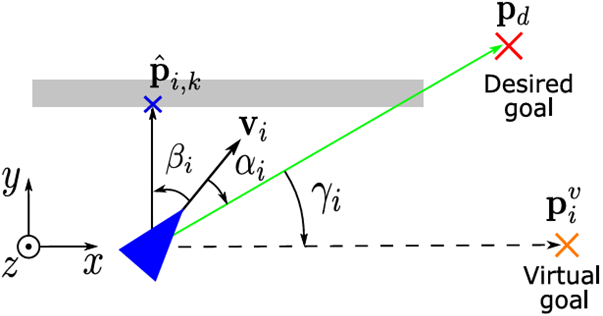
\includegraphics[width=0.4\textwidth]{Pictures/Strategy for tangential navigation.png}
    \caption{Strategy for tangential navigation.}
    \label{fig:Strategy for tangential navigation}
\end{figure}

Nimmt der Roboter zwei Hindernisse (repräsentiert durch zwei Punkte \( \hat{p}_{i,n} \) und \( \hat{p}_{i,n90} \)) 
wahr, die eine Ecke bilden, wendet er das \textit{Corner Avoidance} Manöver an. 
Dabei wird der Rotationswinkel \( \gamma_i \) um einen zusätzlichen Winkel \( \varepsilon_i \) 
ergänzt, der sich aus den Tangentenrichtungen $n$ und $n_{90}$ zu beiden Hindernispunkten 
relativ zum Roboter berechnet ((20) bis (21)). Anschließend wird wieder
ein virtuelles Ziel $p_i^v$ bestimmt, das den Roboter aus der Ecke herausführt (22).

\begin{figure}[h]
    \centering
    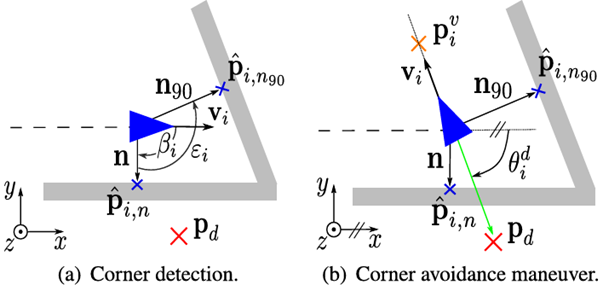
\includegraphics[width=0.4\textwidth]{Pictures/Strategy for corner avoidance.png}
    \caption{Strategy for corner avoidance.}
    \label{fig:Strategy for corner avoidance}
\end{figure}

Wenn der Roboter das Ende eines Hindernisses erreicht hat, führt er eine 
kreisförmige Bewegung um das Ende herum aus. Dazu merkt er sich den letzten 
Hindernispunkt \( \hat{p}_{i,e} \), der in seinem Sensorradius registriert wurde. Anhand  
Gleichung (23) und dem Winkel \( \beta_{i} \), welcher sich durch die tangentiale Navigation 
ergab, berechnet der Roboter in gleichen Abständen virtuelle Ziele (berechnet 
durch Gleichung (24) und repräsentiert durch die Punkte \( p_i^{v1} \), \( p_i^{v2} \) und \( p_d \)) und rotiert um einen 
festen Winkel \( \delta \), bis der Winkel zwischen Bewegungsvektor und virtuelles Ziel kleiner oder gleich \( \delta \) ist (25).

\begin{figure}[h]
    \centering
    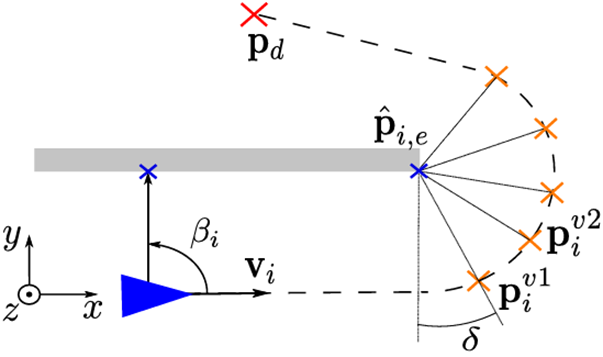
\includegraphics[width=0.4\textwidth]{Pictures/Circular Motion at obstacle endpoint.png}
    \caption{Circular Motion at obstacle endpoint.}
    \label{fig:Circular Motion at obstacle endpoint}
\end{figure}


\section{The proposed navigation approach for a multi-robot system}
Der nun vorgestellte Ansatz erweitert den Navigationsalgorithmus für einzelne Roboter 
um eine Kommunikationsschnittstelle für die kollektive Bewegungsplanung mehrerer 
Roboter. Der Zusammenhalt der Gruppe könnte gefährdet werden, wenn jeder Roboter 
sein eigenes virtuelles Ziel verfolgt. Daher werden Informationen über virtuelle 
Ziele und kritische Punkte (wie in Fig.~\ref{fig:The critical points of obstacles} dargestellt) untereinander ausgetauscht. 
Diese Informationen werden nach Relevanz, Aktualität und dem Prinzip "Erkennung vor 
Kommunikation" priorisiert (erkannte Hindernisse haben dabei Vorrang vor übermittelten 
Informationen aus dem Kommunikationsnetzwerk).
Das Kommunikationsnetzwerk besteht aus Informationspaketen, die sich in drei Typen 
gliedern: Orientierung, Endpunkte und Ecken.

\begin{figure}[h]
    \centering
    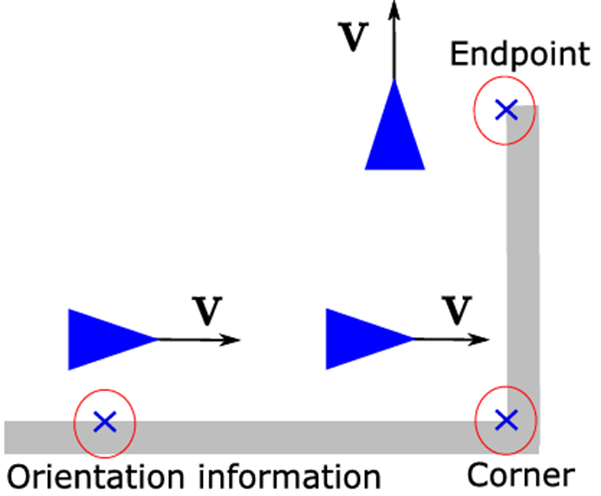
\includegraphics[width=0.25\textwidth]{Pictures/The critical points of obstacles.png}
    \caption{The critical points of obstacles.}
    \label{fig:The critical points of obstacles}
\end{figure}

\textbf{Orientierung (Fig.~\ref{fig:Information about orientation}):} Enthält den Winkel \( \theta_i \) zum aktuellen Ziel, den erkannten 
Punkt \( \hat{p}_{i,k} \) auf dem Hindernis, den aktuellen Status des Roboters (alle Status in Table 1 erklärt) sowie den 
Zeitpunkt der Hinderniserkennung.

\textbf{Endpunkte (Fig.~\ref{fig:Endpoint and corner Information} (a)):} Besteht aus dem zuletzt erkannten Punkt \( \hat{p}_{i,e} \), dem Winkel \( \omega_{i,e} \) 
zwischen dem Normalenvektor vom Roboter zum Hindernis und der x-Achse des inertialen 
Koordinatensystems\footnote{unbeschleunigtes und dem Trägheitsgesetz unterliegendes Koordinatensystem} sowie 
dem Zielwinkel \( \theta_{i,e} \) im Moment der Endpunkterkennung.

\textbf{Ecken (Fig.~\ref{fig:Endpoint and corner Information} (b)):} Umfasst den Zielwinkel beim Eintritt (\( \theta_{i,\mathrm{ent}} \)) und Austritt 
(\( \theta_{i,\mathrm{ex}} \)) aus der Ecke sowie den Eckpunkt \( \hat{p}_{i,c} \), der als Schnittpunkt aus den
erkannten Hindernislinien berechnet wird.

Bevor ein Roboter eine Aktion anhand der gegebenen Orientierungsinformationen aus 
dem Kommunikationsnetzwerk ausführt, berechnet dessen Relevanz über die Funktion \( \mathrm{rel} \), 
welche im Intervall \( ]-\infty, 10] \) liegt. Dabei steht \( \mathrm{rel}=10 \) für eine 
sehr relevante und \( \mathrm{rel} \leq 0 \) für eine zu ignorierende Information. 
Unterschieden wird dabei wie folgt:
\begin{itemize}
    \item \textbf{Alter der Information:}
    Die Gleichung
    \begin{equation}
        \mathrm{rel}_t = 10 - \frac{10 \cdot (t_k - \hat{t}^c)}{d_t}
        \label{eq:5}
    \end{equation}
    bestimmt: je älter die Information, desto unwichtiger ist sie, mit 
    der aktuellen Zeit \( t_k \) und der Registrierungszeit \( \hat{t}^c \) der Information von einem 
    anderen Roboter und \( d_t \in \mathbb{R} \) eine Konstante, die \( \mathrm{rel_t} \) ab einer
    bestimmten Zeit negativ werden lässt.
    
    \item \textbf{Distanz vom Hindernis:}
    Sollte das Hindernis in Bewegungsrichtung liegen, 
    so ermittelt sich die Relevanz der Distanz mit 
    \begin{equation}
        \mathrm{rel}_{\mathrm{dist}} = 10 - \frac{10 \cdot \| \hat{p}^c - p_i \|}{d_x}
        \label{eq:6}
    \end{equation}
    mit \( d_x \in \mathbb{R} \) die maximale Distanz und \( \| \hat{p}^c - p_i \| \) der Abstand des Roboters ($p_i$) 
    zum Hindernis ($\hat{p}^c$). Liegt es dahinter, dann mit
    \begin{equation}
        \mathrm{rel}_{\mathrm{dist}} = - \frac{10 \cdot \| \hat{p}^c - p_i \|}{d_x}
        \label{eq:7}
    \end{equation}
    und sollten keine Orientierungsinformationen gegeben sein, so 
    ist \( \mathrm{rel}_{\mathrm{dist}} = 0 \).
    
    \item \textbf{Relevanz der Orientierung basierend auf dem vorherigen Zeitschritt:}
    Jeder Roboter erwartet für jeden Zeitschritt nur kleine Änderungen in der tangentialen 
    Navigation. Die Gleichung 
    \begin{equation}
        \mathrm{rel}_{\mathrm{exp}} = 10 - \frac{10 \cdot | \theta_i(t_k) - \theta^c |}{d_\theta}
        \label{eq:8}
    \end{equation}
    beschreibt die Relevanz der erwarteten Orientierung, wobei 
    \( |\theta_i(t_k) - \theta^c| \) der Vergleich mit der aktuellen Zielorientierung ($\theta_i(t_k)$) und 
    der neuen Orientierung ($\theta^c$) ist und \( d_\theta \) die maximal erlaubte Winkeldifferenz, sodass
    \( \mathrm{rel}_{\mathrm{exp}} > 0 \).
    
    \item \textbf{Auswertung des Senders:}
    Empfangenen Informationen sind relevanter, wenn der Sender der Besitzer dieser Informationen ist.
    \begin{equation}
        \mathrm{rel}_o =
        \begin{cases}
        10, & \text{wenn direkt gesendet}\\
        0, & \text{wenn nur weitergeleitet}
        \end{cases}
        \label{eq:9}
    \end{equation}
    
    \item \textbf{Auswertung anhand des Status:}
    Aktionen die den Roboter neu ausrichten, werden mit höchster Relevanz bewertet. Alle \textit{status} sind in Tabelle 1
    nachsehbar.
    \begin{equation}
        \mathrm{rel}_{\mathrm{type}} =
        \begin{cases}
        10, & \text{if } status^c = 4 \vee status^c = 3 \\
        5,  & \text{if } status^c = 1 \\
        0,  & \text{otherwise}
        \end{cases}
        \label{eq:10}
    \end{equation}
\end{itemize}

Die endgültige Relevanz ergibt sich aus der Gleichung
\begin{equation}
    \scalebox{1.15}{$\overline{\mathrm{rel}}_n = \frac{c_{\mathrm{type}} \cdot \mathrm{rel}_{\mathrm{type}} + c_o \cdot \mathrm{rel}_o + c_{\mathrm{exp}} \cdot \mathrm{rel}_{\mathrm{exp}} + c_{\mathrm{dist}} \cdot \mathrm{rel}_{\mathrm{dist}} + c_t \cdot \mathrm{rel}_t}{c_{\mathrm{type}} + c_o + c_{\mathrm{exp}} + c_{\mathrm{dist}} + c_t}$}
    \label{eq:11}
\end{equation}
wobei die maximale Relevanz durch 
\begin{equation}
    \mathrm{rel}_{\mathrm{max}} = \underset{\mathrm{rel}_n \in \mathcal{R}_i}{\mathrm{argmax}}(\mathrm{rel}_n)
    \label{eq:12}
\end{equation}
berechnet wird, mit $n \in \mathcal{S}_i$, die Menge aller aus dem Netzwerk erhaltene Informationspakete und 
$\mathcal{R}_i$ die Menge aller aus den Informationspaketen entnommenen Relevanzwerte für Roboter $i$.

Ein Informationspaket ist für einen Roboter schließlich relevant, wenn die Bedingung
\begin{equation}
    \mathrm{rel}_n \geq 0.95 \cdot \mathrm{rel}_{\mathrm{max}}
    \label{eq:13}
\end{equation}
erfüllt ist. Er passt daraufhin seine 
Bewegungsrichtung für den nächsten Zeitschritt an. Sollten mehrere Informationspakete 
diese Bedingung erfüllen, wird der Mittelwert daraus bestimmt.

Zu übermittelten Ecken oder Endpunkten, prüft der Roboter seine Distanz $d_s$ mit
\begin{equation}
    \begin{split}
    d_s \leq \| p_i - \hat{p}_c^c \| \leq R_{\mathrm{rel}},\\
    d_s \leq \| p_i - \hat{p}_e^c \| \leq R_{\mathrm{rel}},
    \end{split}
    \label{eq:14}
\end{equation}
und sieht diese Punkte dann als seine eigenen Hindernispunkte an, sollten 
sie innerhalb der maximalen Distanz \( R_{\mathrm{rel}} \in \mathbb{R} \) liegen.

\begin{figure}[h]
    \centering
    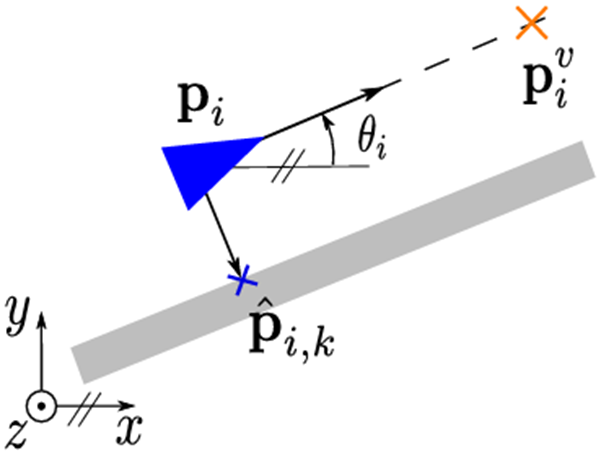
\includegraphics[width=0.25\textwidth]{Pictures/Information about orientation.png}
    \caption{Information about orientation.}
    \label{fig:Information about orientation}
\end{figure}

\begin{figure}[h]
    \centering
    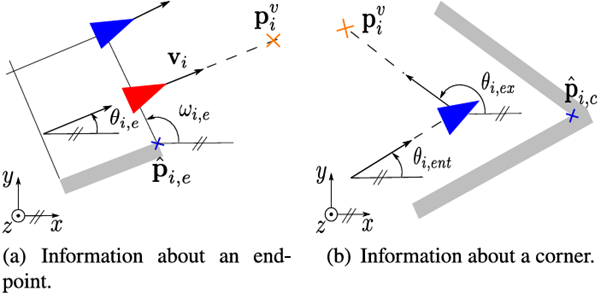
\includegraphics[width=0.4\textwidth]{Pictures/Endpoint and corner Information.png}
    \caption{Endpoint and corner Information.}
    \label{fig:Endpoint and corner Information}
\end{figure}


\section{Collective navigation using shared information}
In diesem Abschnitt wird erklärt, wie die Verfahren eines einzelnen Roboters auf ein 
Multi-Roboter-System erweitert werden können. Dazu sind 7 Status definiert, in dem 
sich ein Roboter befinden kann, wobei sich jeder zum Start im Status 0 befindet 
(Erklärungen und Abhängigkeiten in Appendix A).

\subsection*{Collective tangential navigation}
Die kollektive tangentiale Navigation umfasst die Status 1, 4 und 5. Erkennt ein 
Roboter ein Hindernis innerhalb seiner Wahrnehmungsreichweite \( r_{\mathrm{tan}} \), so leitet er, 
wie beim Einzelroboter, die tangentiale Navigation ein. Diese Aktion wird als 
Status 1 bezeichnet. Die dabei ermittelten Informationen werden an benachbarte 
Roboter weitergeleitet (Algorithmus 2).
Da die Steuergröße \( u_i^\alpha \) gemäß Gleichung (8) dazu führen kann, dass sich Roboter 
durch Abstoßung senkrecht zum Hindernis voneinander entfernen und so unbeabsichtigt 
ein Wechsel von \textbf{Status 0} auf \textbf{1} ausgelöst werden könnte, wurde eine 
Ignoranz-Bedingung~(\ref{eq:15}) 
entwickelt, damit Roboter Hindernisse ignorieren können.
\begin{equation}
    \begin{split}
    (|\upsilon_i| > 90^\circ \wedge |\beta_i| > 91^\circ) \vee \\
    \| \hat{p}_{i,k} - p_i \| > 0.3 \cdot (r_{\text{tan}} - d_s) + d_s
    \end{split}
    \label{eq:15}
\end{equation}

Wird ein Roboter durch neue Informationen aus dem Kommunikationsnetzwerk in eine 
ungünstige Ausrichtung gebracht und der Unterschied zwischen seiner aktuellen Bewegungs- 
und Zielausrichtung größer als 45° ist, so wechselt er in 
den Status 4 (Algorithmus 5), um seine Ausrichtung zu korrigieren.
Berechnet ein Roboter aufgrund empfangener Informationen ein virtuelles Ziel mittels 
Gleichung 38, befindet er sich im Status 5 (Algorithmus 6).
Um zu verhindern, dass Roboter Hindernisendpunkte zu spät erkennen, wenn diese nur 
von anderen benachbarten Robotern erfasst wurden, wird eine Distanzabschätzung mit 
einer Fallunterscheidung (Bedingung 39) vorgenommen. Damit kann der Roboter anhand 
der Entfernung zum Hindernis oder zu einer projizierten Position seine 
Zielausrichtung rechtzeitig anpassen und so Verzögerungen im Bewegungsablauf vermeiden.

\subsection*{Collective corner avoidance}
Nähert sich ein Roboter einer Ecke, kann er sie, wie in 
Abschnitt~\ref{sec:Single robot navigation} beschrieben, 
umfahren und dabei zusätzlich Informationen aus dem Kommunikationsnetzwerk nutzen. 
Diese Aktion wird als Status 3 bezeichnet.

Damit dabei keine möglichen Durchgänge 
(z. B. zwischen zwei Hindernissen) übersehen werden, prüft der Roboter zuvor die 
Bedingung 40. Nur wenn diese erfüllt ist, wird die Ecke als solche erkannt.
Anschließend definiert der Roboter ein neues virtuelles Ziel und wechselt in Status 4, 
um sich neu auszurichten. Gleichzeitig sendet er Informationen über die erkannte Ecke 
an die benachbarten Roboter.
Wird die Bedingung 40 jedoch nicht erfüllt, verbleibt der Roboter zunächst im 
Wartezustand (Status 6). In diesem Zustand überwacht er das Kommunikationsnetzwerk 
seiner Nachbarn. Wird dabei eine Information mit Status 3 oder 4 als relevant 
eingestuft, übernimmt der Roboter sie und verlässt den Wartezustand. Gibt es 
stattdessen relevante Informationen mit Status 1 oder 2, passt er sich entsprechend 
an und folgt entweder der tangentialen Navigation oder dem Manöver an einem Hindernisendpunkt.

\subsection*{Collective motion at obstacle extremities}
Erkennt ein Roboter den Endpunkt eines Hindernisses, folgt er virtuellen Zielpositionen 
auf einem kreisförmigen Pfad (Status 2), wie in 
Abschnitt~\ref{sec:Single robot navigation} beschrieben. Jeder 
Roboter legt individuelle Ziele auf diesem Pfad fest und teilt Informationen zum 
Endpunkt in seinem Netzwerk (Fig.~\ref{fig:Collective maneuver at an obstacle endpoint}).

\begin{figure}[h]
    \centering
    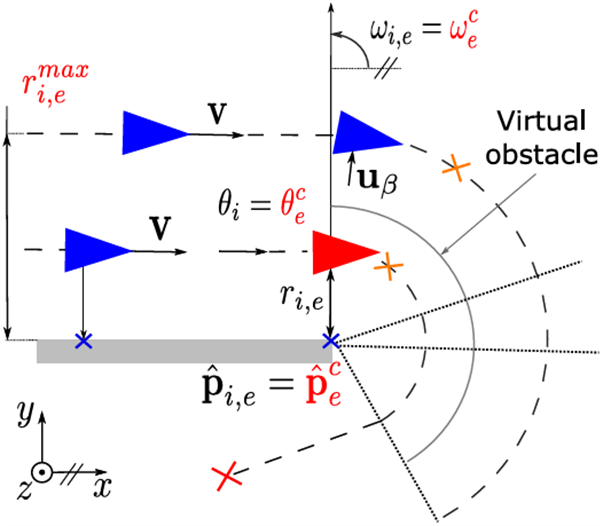
\includegraphics[width=0.4\textwidth]{Pictures/Collective maneuver at an obstacle endpoint.png}
    \caption{Collective maneuver at an obstacle endpoint.}
    \label{fig:Collective maneuver at an obstacle endpoint}
\end{figure}

Nach Erhalt der Endpunktdaten prüft ein Roboter seine 
Position durch orthogonale Projektion auf eine virtuelle Startlinie, 
bevor er die Kreisbewegung beginnt. Sollte der Roboter diese Startlinie noch nicht 
erreicht haben (Bedingung 42), setzt er weitere tangentiale Ziele und passt seine 
Geschwindigkeit an die Mindestgeschwindigkeit für die Kreisbewegung an 
(Gleichung 43 und 44). Erreicht er die Startlinie, beginnt die Kreisbewegung 
entsprechend des in 
Abschnitt~\ref{sec:Single robot navigation} vorgestellten Schemas.

Während der Bewegung stellt eine Komponente aus Gleichung 8 sicher, dass der Roboter 
sein Ziel auf dem kreisförmigen Pfad erreicht. Überschreitet ein Roboter sein 
virtuelles Ziel, wird eine neue Zielposition berechnet.

Die Roboter bewegen sich auf individuellen Kreisbahnen mit 
unterschiedlichen Radien, wodurch innere Kreise kürzere Wege bedeuten. 
Der Geschwindigkeitskonsens basiert bei der Kreisbewegung auf gleichen 
Winkelgeschwindigkeiten. Dafür wird eine minimale Winkelgeschwindigkeit (45) 
festgelegt und die Steuergröße aus Gleichung 8 für eine angepasste Steuergröße 
aus Gleichung 46 und 47 ersetzt. Dadurch können die Roboter gleichförmig das 
Hindernisende umkreisen.

\subsection*{Conditional Braking}

Wenn mehrere Roboter einer Gruppe eine kreisförmige Bewegung um ein Hindernis 
ausführen, können durch unterschiedliche Zeitpunkte beim Verlassen der Kreisbahn 
Geschwindigkeitsunterschiede entstehen, die zum Auseinanderreißen der Gruppe führen. 
Um dies zu verhindern, werden Roboter, die das Hindernis bereits passiert haben, 
abgebremst. Dieses Abbremsen bleibt solange aktiv, bis der letzte Roboter der 
Gruppe die Kreisbahn verlassen hat.

Zur Bestimmung dieses letzten Roboters wird ein neues Koordinatensystem definiert, 
dessen Ursprung im Endpunkt des Hindernisses liegt. In diesem System wird die 
Position jedes Roboters auf die x-Achse projiziert. Anhand dieser projizierten 
Positionen und über Gleichung 53 betrachten die Roboter ihre Nachbarschaft und 
identifizieren den Roboter, der am weitesten hinten liegt.

Über eine Gossip-ähnliche 
Kommunikation\footnote{lokaler, dezentraler und iterativer Informationsaustausch}
wird die gesamte Gruppe über diesen Kandidaten informiert, 
bis alle Roboter den globalen hintersten Roboter ermittelt haben. Sobald 
dieser Roboter seine Kreisbewegung beendet hat, sendet er ein Reset-Signal, 
um das Bremsen der restlichen Roboter aufzuheben und die Gruppenbewegung 
wieder zu synchronisieren.

\subsection*{Watchdog timer}
Fällt die Geschwindigkeit eines Roboters unter einen definierten Schwellenwert, 
aktiviert er einen selbstüberwachenden Mechanismus, den \textit{Watchdog Timer}. 
Dabei speichert der Roboter seine aktuelle Position und den aktuellen Zeitpunkt. 
Der Timer wird wieder deaktiviert, sobald sich der Roboter innerhalb der 
folgenden Zeitschritte um mehr als einen festgelegten Schwellenwert bewegt 
(Roboter nimmt an einen möglichen Deadlock\footnote{ausweglose Situation} verlassen zu haben). 
Bewegt sich der Roboter jedoch über einen Zeitraum von 15 Sekunden kaum 
und wurde der Timer nicht deaktiviert, wechselt er automatisch in Status 0 
und bewegt sich in Richtung desired goal. Diese Maßnahme kann zwar zu einer 
Fragmentierung der Gruppe führen, stellt jedoch sicher, dass jeder Roboter 
das desired goal erreicht.


\section{Simulation results}
Die Simulationsergebnisse werden anhand von zwei Szenarien dargestellt: 
einem mit einem Zickzack-Hindernis und einem mit einem Korridor mit Hindernissen. 
In beiden Fällen werden zwölf Roboter zufällig 
innerhalb eines Startbereichs positioniert, jeweils ohne Anfangsgeschwindigkeit. 
Zusätzlich wird ein desired goal (als rotes Kreuz markiert) definiert.

Die Roboter werden in den Abbildungen als schwarze Dreiecke dargestellt. 
Ihre Bewegung wird durch eine bunte Linie hinter den Dreiecken visualisiert, 
die Bewegungsrichtung entspricht der Ausrichtung der Dreiecksspitze. Die schwarzen 
Linien zwischen den Robotern zeigen das aktive Kommunikationsnetzwerk an. 
Die Abbildungen geben Momentaufnahmen zu bestimmten Zeitpunkten bzw. 
bei relevanten Ereignissen während der Simulation wieder.

Im ersten Szenario (Fig.~\ref{fig:Sequential snapshots of 12 agents collectively navigating through a zigzag obstacle}) zeigen sich folgende Abläufe:
\begin{itemize}
\item (a): Erkennung eines Hindernisses und Beginn der tangentialen Navigation
\item (b): Erkennung eines Eckpunktes und Ausführung des \textit{corner avoidance maneuvers}
\item (c) und (d): Erkennung eines Endpunktes und Einleitung der kreisförmigen Bewegung um das Hindernis
\item (e): Annäherung der Roboter an das Hindernis zur Optimierung der Navigation mithilfe von Gleichung 39
\item (f): Erreichen des gewünschten Zielpunkts
\end{itemize}

Im zweiten Korridor-Szenario (Abbildung 15) kommen dieselben Verfahren zum Einsatz.

\subsection*{Guideline for parameter choice}
Die Parameter der Relevanzfunktion (Gleichung 32) sollten in Abhängigkeit des 
jeweiligen Szenarios gewählt werden. Ein globales Verhalten des 
Multi-Roboter-Systems, bei dem alle Roboter nahezu gleichzeitig identische 
Aktionen ausführen, ist dabei für kleinere Systeme mit sechs bis zwölf 
Robotern geeignet, wenn deren Verteilung im Verhältnis zu den Hindernissen 
gering ist. In diesem Fall sollten die Relevanz der Zeit des Informationspakets 
(\texttt{relt}) und der Relevanz des Aktionsstatus (\texttt{reltype}) höher 
gewichtet werden als die übrigen Werte, damit Roboter gleichartig und möglichst
synchron auf aktuelle Ereignisse im Kommunikationsnetzwerk reagieren.

Bei steigender Anzahl von Robotern oder einer dichteren Hinderniskonstellation 
kann ein solches globales Verhalten jedoch problematisch sein, da einzelne 
Roboter gleichzeitig mehrere relevante Informationspakete erhalten könnten. 
In diesen Situationen sollten Roboter stärker auf ihre eigene Position und lokale 
Informationen achten. Dazu werden die Relevanz des Abstands zum Hindernis 
(\texttt{reldist}), die Relevanz der erwarteten Orientierung für die nächste Aktion 
(\texttt{relexp}) sowie die Relevanz des Senders der Information (\texttt{relo}) 
höher gewichtet als \texttt{relt} und \texttt{reltype}.

Die Effekte dieser unterschiedlichen Gewichtungen zeigen sich in den folgenden Abbildungen:
\begin{itemize}
\item Abbildung 16 zeigt ein \textit{squeezing maneuver}, bei dem sich die 
Robotergruppe zwischen zwei kreisförmigen Hindernissen hindurch bewegt.
\item In Abbildung 17 ist zu erkennen, wie ein halbkreisförmiges Hindernis 
die Gruppe aufteilt. Die Roboter korrigieren daraufhin ihre Bewegungsrichtung, 
indem sie ihren aktuellen Aktionsstatus überprüfen und anpassen.
\item Abbildung 18 veranschaulicht, dass durch die priorisierte 
Hindernisvermeidung eine Fragmentierung der Gruppe auftritt. 
Dennoch erreichen letztlich alle Roboter das gewünschte Ziel.
\end{itemize}


\section{Conclusion}
In dieser Arbeit wurde ein Verfahren zur kollektiven Navigation autonomer Roboter 
in unbekannten Umgebungen entwickelt. Der Ansatz kombiniert eine tangentiale 
Umgehungsstrategie mit dem Austausch lokaler Umgebungsinformationen über ein 
Kommunikationsnetz. Kollisionsfreie und koordinierte Bewegungen der Roboter 
werden durch künstliche Potentialkräfte ermöglicht, die ein schwarmähnliches 
Verhalten erzeugen. Durch eine gezielte Anpassung der Parameter der 
Relevanzfunktion und Gewichtung kann eine Fragmentierung der Gruppe 
vermieden werden. Einzelne Roboter behalten dabei die Fähigkeit, ihr Ziel 
auch ohne Gruppenanschluss zu erreichen. Für holonomische\footnote{Position 
kann unabhängig der Ausrichtung geändert werden} Roboter ist dabei 
insbesondere ein ausreichend großer Sicherheitsabstand sowie eine reduzierte 
Geschwindigkeit entscheidend. Zukünftige Arbeiten sollen sich mit der 
Umsetzung in Echtzeit, der Optimierung der drahtlosen Kommunikation und 
alternativen Netzwerkstrukturen für die Roboter befassen.


\section*{Appendix}
\subsection*{Equations, functions and conditions}

\subsection*{Figures and tables}
\begin{figure*}[]
    \centering
    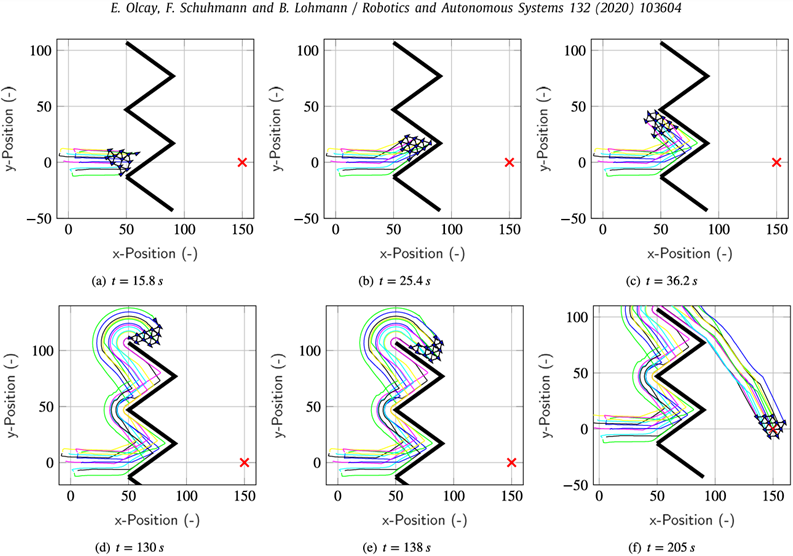
\includegraphics[width=1.0\textwidth]{Pictures/Sequential snapshots of 12 agents collectively navigating through a zigzag obstacle.png}
    \caption{Sequential snapshots of 12 agents collectively navigating through a zigzag obstacle.}
    \label{fig:Sequential snapshots of 12 agents collectively navigating through a zigzag obstacle}
\end{figure*}


\bibliographystyle{IEEEtran}
\bibliography{IEEEabrv,literature}

\end{document}
